\chapter{System Validation}\label{ch:validation}

This chapter presents the validation of the proposed solution.
The validation process is described into different sections, each addressing different components of the system.
Section~\ref{sec:meth} outlines the methodology used for validation.
Section ~\ref{sec:experimental-setup} presents the experimental setup.
In Section ~\ref{sec:component-testing}, each component is individually tested, as well as its proper functioning in the system.
Section~\ref{sec:use_case} presents a specific use case to demonstrate the system's functionality.
Finally, Section~\ref{sec:discuss} provides a discussion of the results and insights gained from the validation process.

\section{Methodology}\label{sec:meth}
We have divided our tests into three categories: Component Testing, Interoperability Testing and Use Case Validation.
The first was used to validate the proper functioning of each component, with a performance evaluation when possible.
The second category serve to determine if the components were working jointly properly.
The last seek to validate the proposed system in a reference scenario.
We have conducted functional validation using tools such as ping and Iperf~\cite{iperf}.
When applicable, the performance was evaluated.
Following that, the last set of tests consisted of a use case validation in various scenarios.

\section{Experimental Setup}\label{sec:experimental-setup}
This section presents the experimental setup.
Figure~\ref{fig:setup} shows a photograph of the experimental scenario.

\begin{figure}[H]
    \centering
    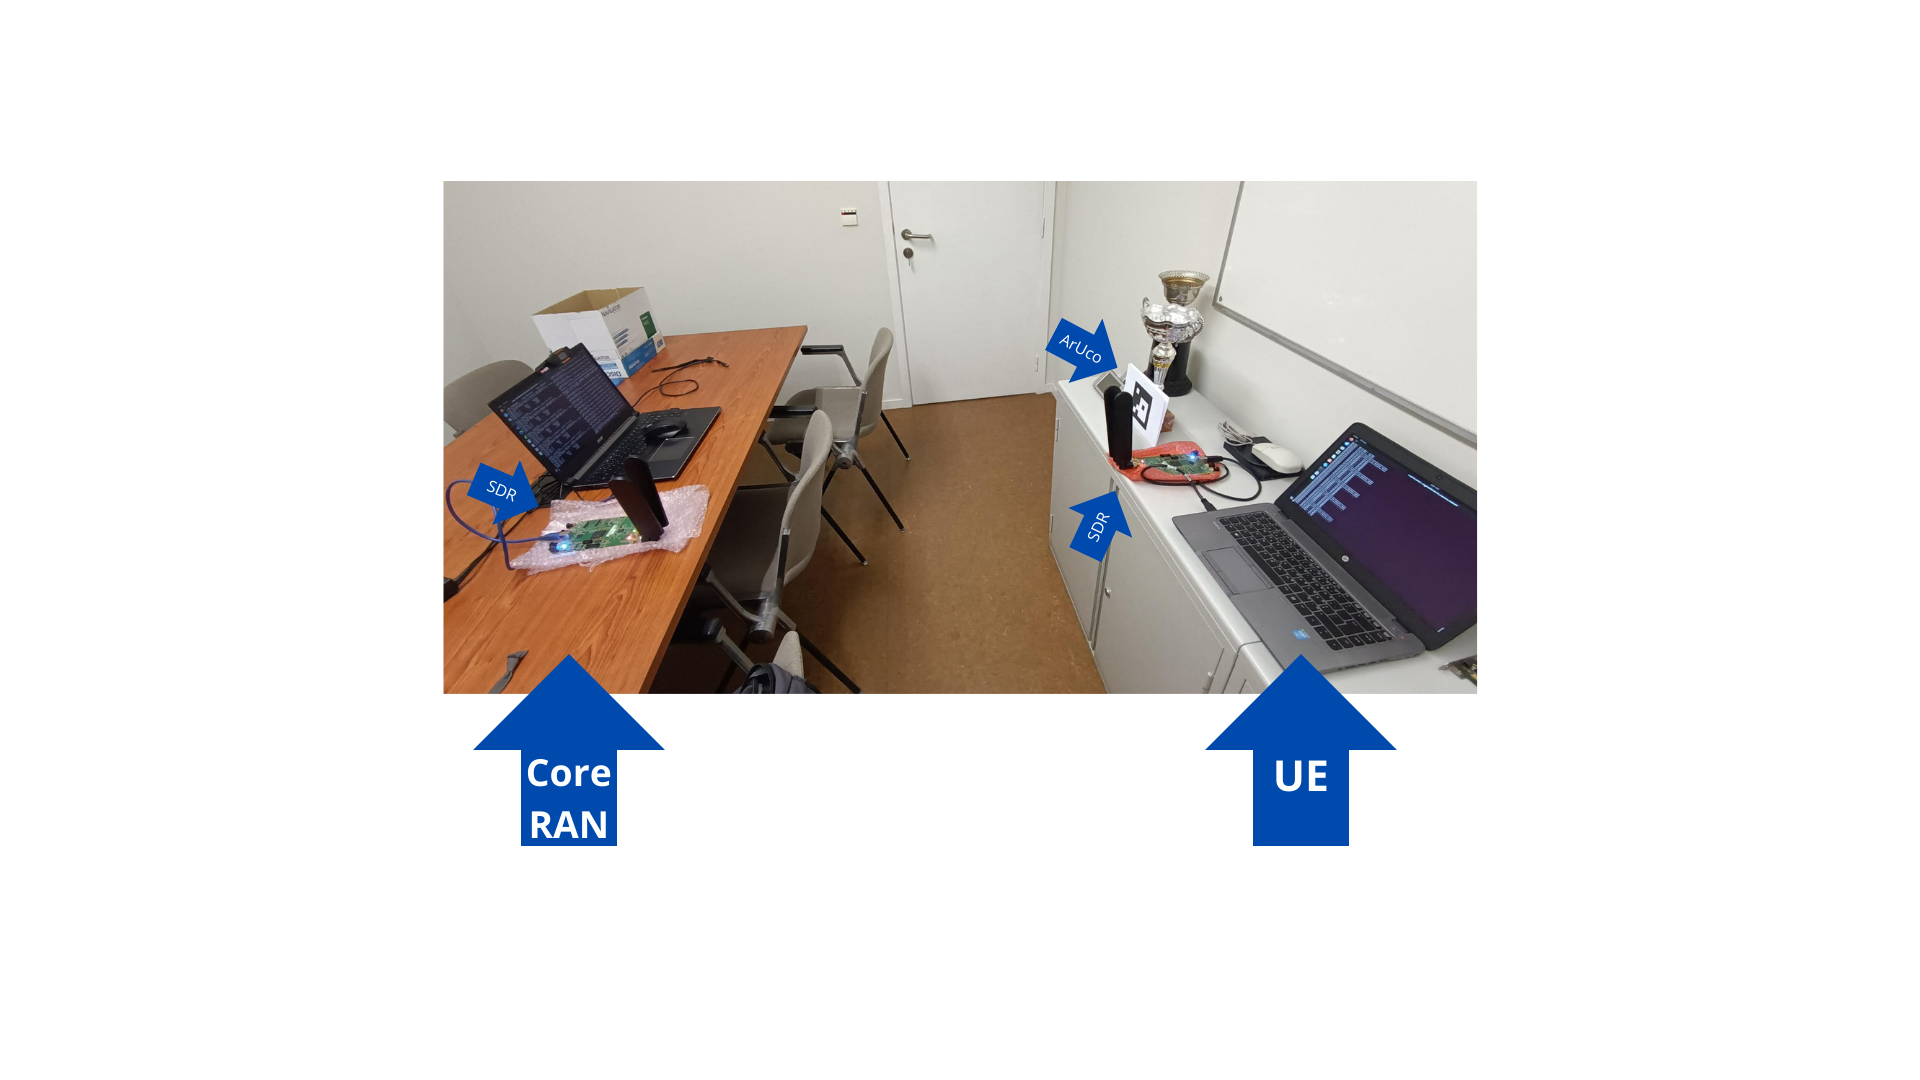
\includegraphics[width=\linewidth]{figures/setup}
    \caption{Experimental setup.}
    \label{fig:setup}
\end{figure}

In order to produce a higher attention introduced by an obstacle, we have used an RF absorbing material.
Since we are not using mmWaves, the attenuation introduced by obstacles is not so great, and so to simulate this scenario, we used it.
The person,i.e.\ the obstacle holds the material when passing between the gNB and UE\@.
Figure~\ref{fig:foam} shows the material utilized.

\begin{figure}[H]
    \centering
    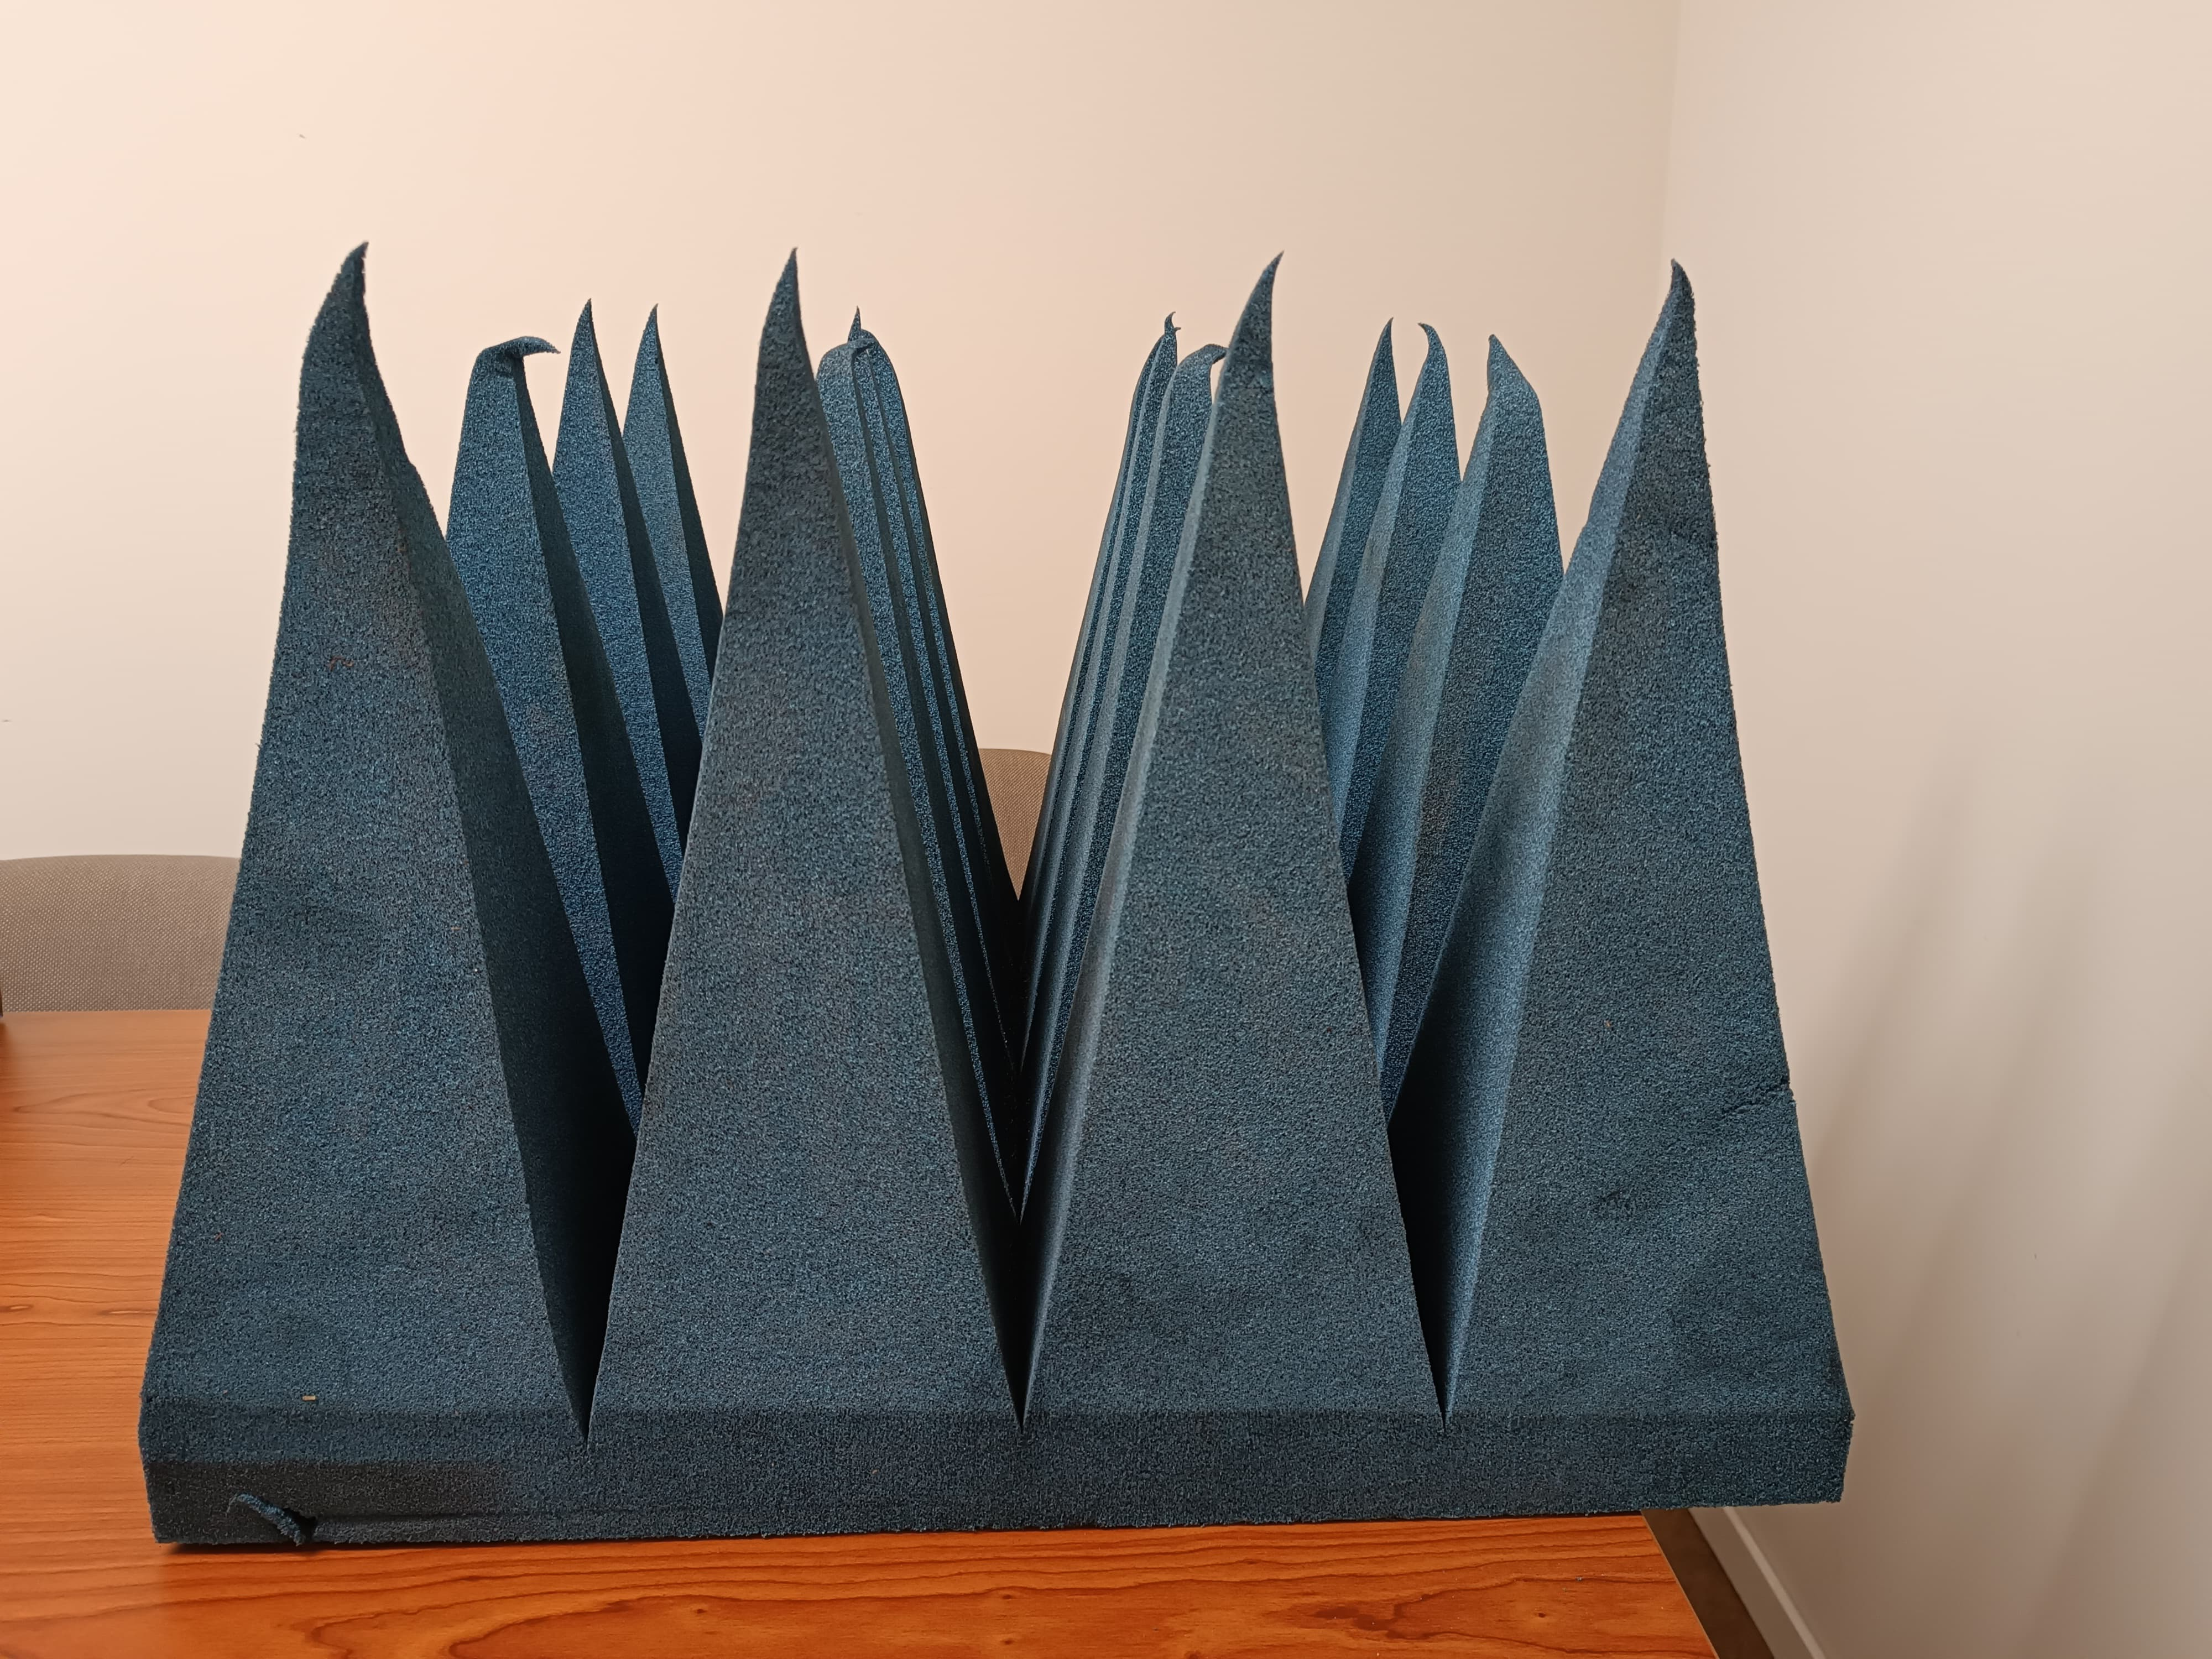
\includegraphics[width=0.5\linewidth]{figures/foam}
    \caption{}
    \label{fig:foam}
\end{figure}



\section{Component and interoperability testing}\label{sec:component-testing}


\subsection{Core Network}\label{subsec:core_network}
In this section, the Core Network configuration and validation are discussed.
It includes the setup of network elements, their interactions, and performance metrics.
In order to make sure that all Core Network components are working properly, we performed a test.
The deployment of the Core Network is done through Docker containers.
Figure~\ref{fig:core_init} presents the command for running the Core Network setup script.
After the initialization of the Docker containers, it is possible to see the logs of the setup script, indicating the successful initialization.

\begin{figure}[H]
    \centering
    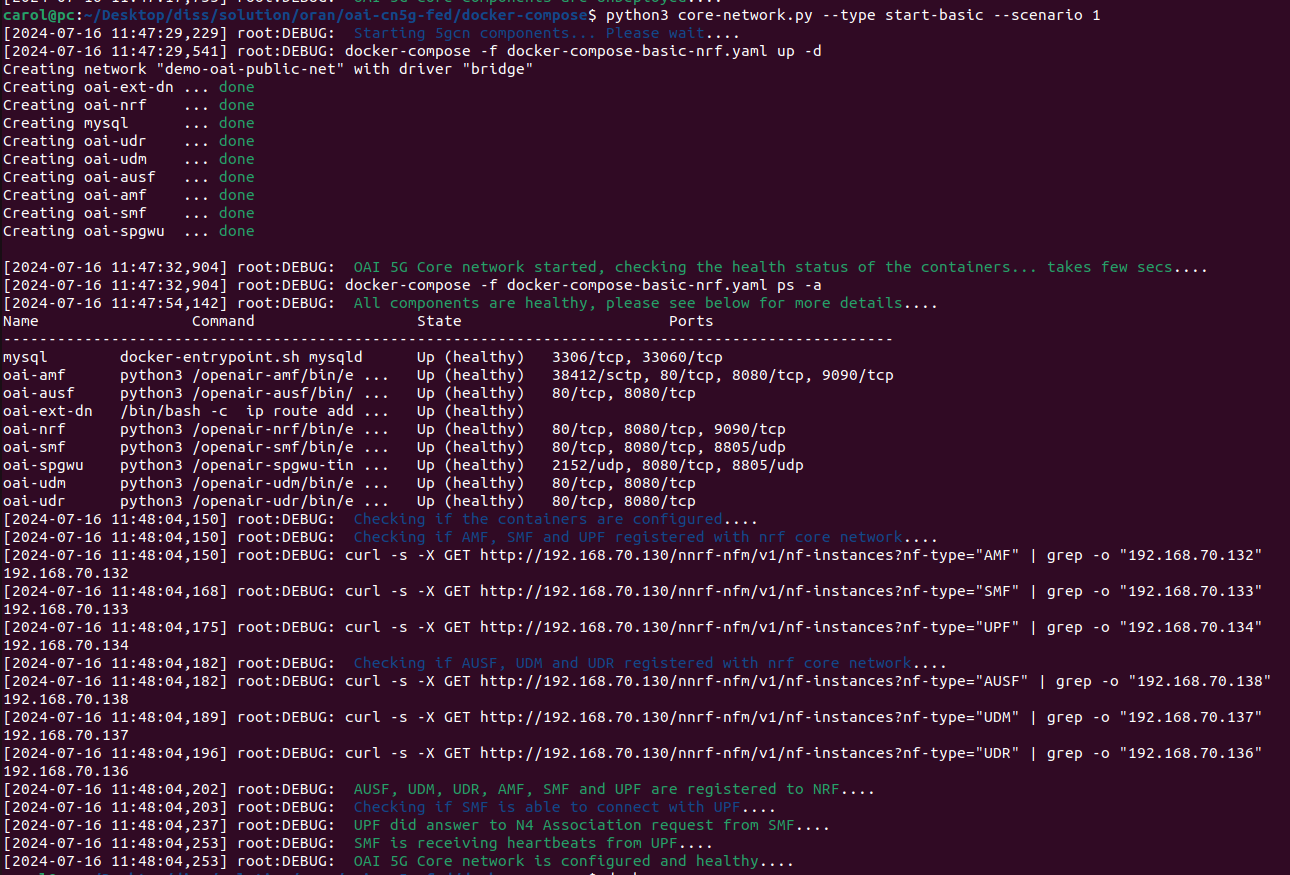
\includegraphics[width=0.5\linewidth]{figures/core_init}
    \caption[Initialization of the Core Network]{Initialization of the Core Network.}
    \label{fig:core_init}
\end{figure}

In order to confirm the correct deployment, the interface \textit{demo-oai} must appear when running the \textit{ifconfig} command.

Then, we verified that all the containers had connectivity using the interface created in the Host OS, using the ping tool,as shown by Figures ~\ref{fig:ping_core1} and ~\ref{fig:ping_core2}.
Each interface sends requests to each network component according to the table~\ref{tab:ip_core}.
Successfully concluding this tests ensures that the 5G Core Network is operational.

\begin{figure}[H]
\centering
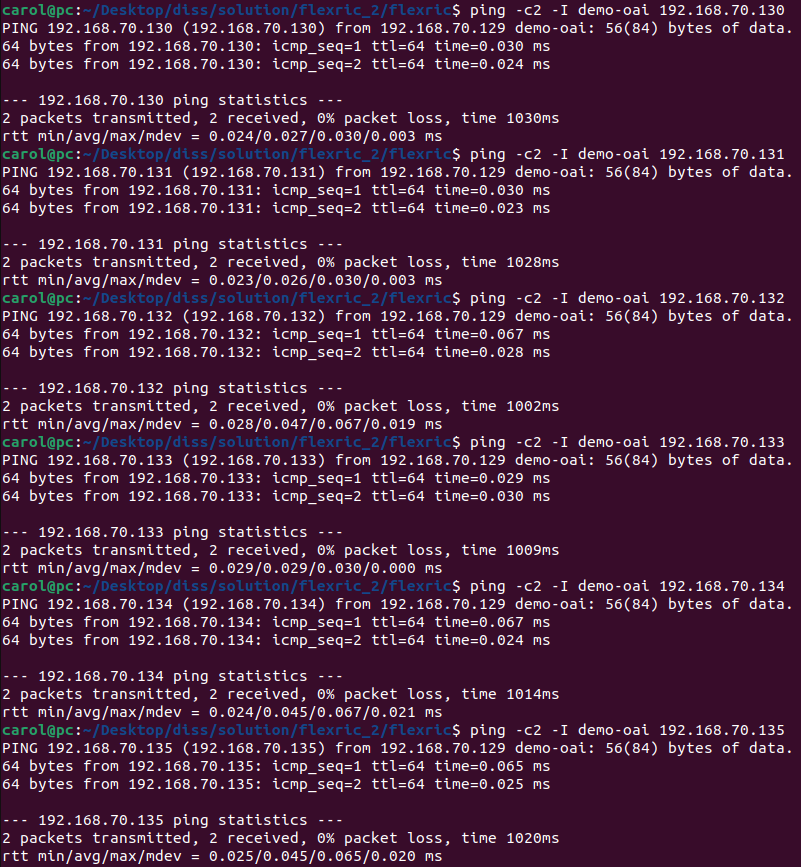
\includegraphics[width=0.5\linewidth]{figures/ping_core_1}
\caption[Pinging Core Network components from Host OS
interface]{Pinging Core Network components from Host OS
interface.}
\label{fig:ping_core1}
\end{figure}

\begin{figure}[H]
    \centering
    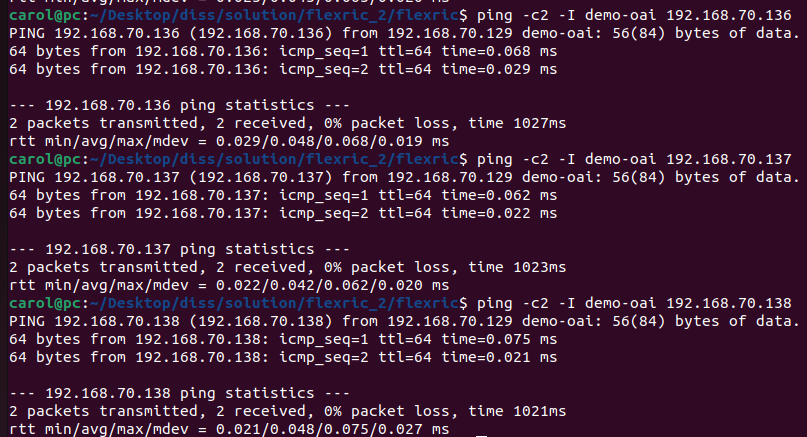
\includegraphics[width=0.5\linewidth]{figures/ping_core_2}
    \caption[Pinging Core Network components from Host OS
    interface]{Pinging Core Network components from Host OS
    interface.}
    \label{fig:ping_core2}
\end{figure}




\subsection{FlexRIC}\label{subsec:flexric2}
As for the FlexRIC deployment, it is simply necessary to assure its correct launch.
Upon launching, it awaits for incoming connection requests from an E2 Node.
Figure~\ref{fig:near-rt-ric} shows the initialization of the FlexRIC\@.

\begin{figure}[H]
    \centering
    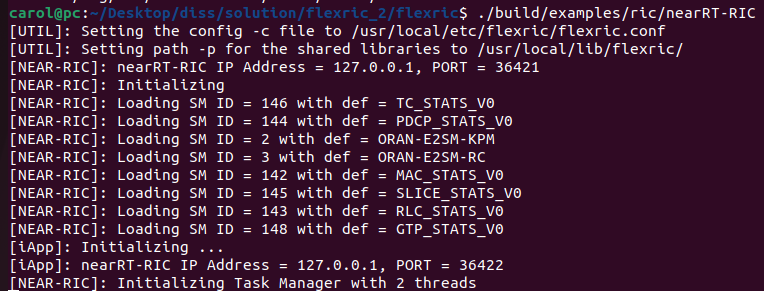
\includegraphics[width=0.5\linewidth]{figures/flexric_init}
    \caption{Initialization of FlexRIC's executable.}
    \label{fig:near-rt-ric}
\end{figure}

When it is properly launched, the gNB can be initialized.

\subsection{gNB}\label{subsec:gnb}
To ensure the correct functioning of the gNB, it should be registered in the 5G Core Network, connected to the FlexRIC and registered as a E2 node.
They need to be validated separately since the connections are independent.

After executing the command to launch the gNB\@, it is possible to verify the proper operation of the SDR by its Light-Emitting Diodes (LEDs).
Three LEDs blue, green and red indicate the powering of the SDR, the transition, and the reception of radio signals respectively, depicted by Figure~\ref{fig:usrp_working}.

\begin{figure}[H]
    \centering
    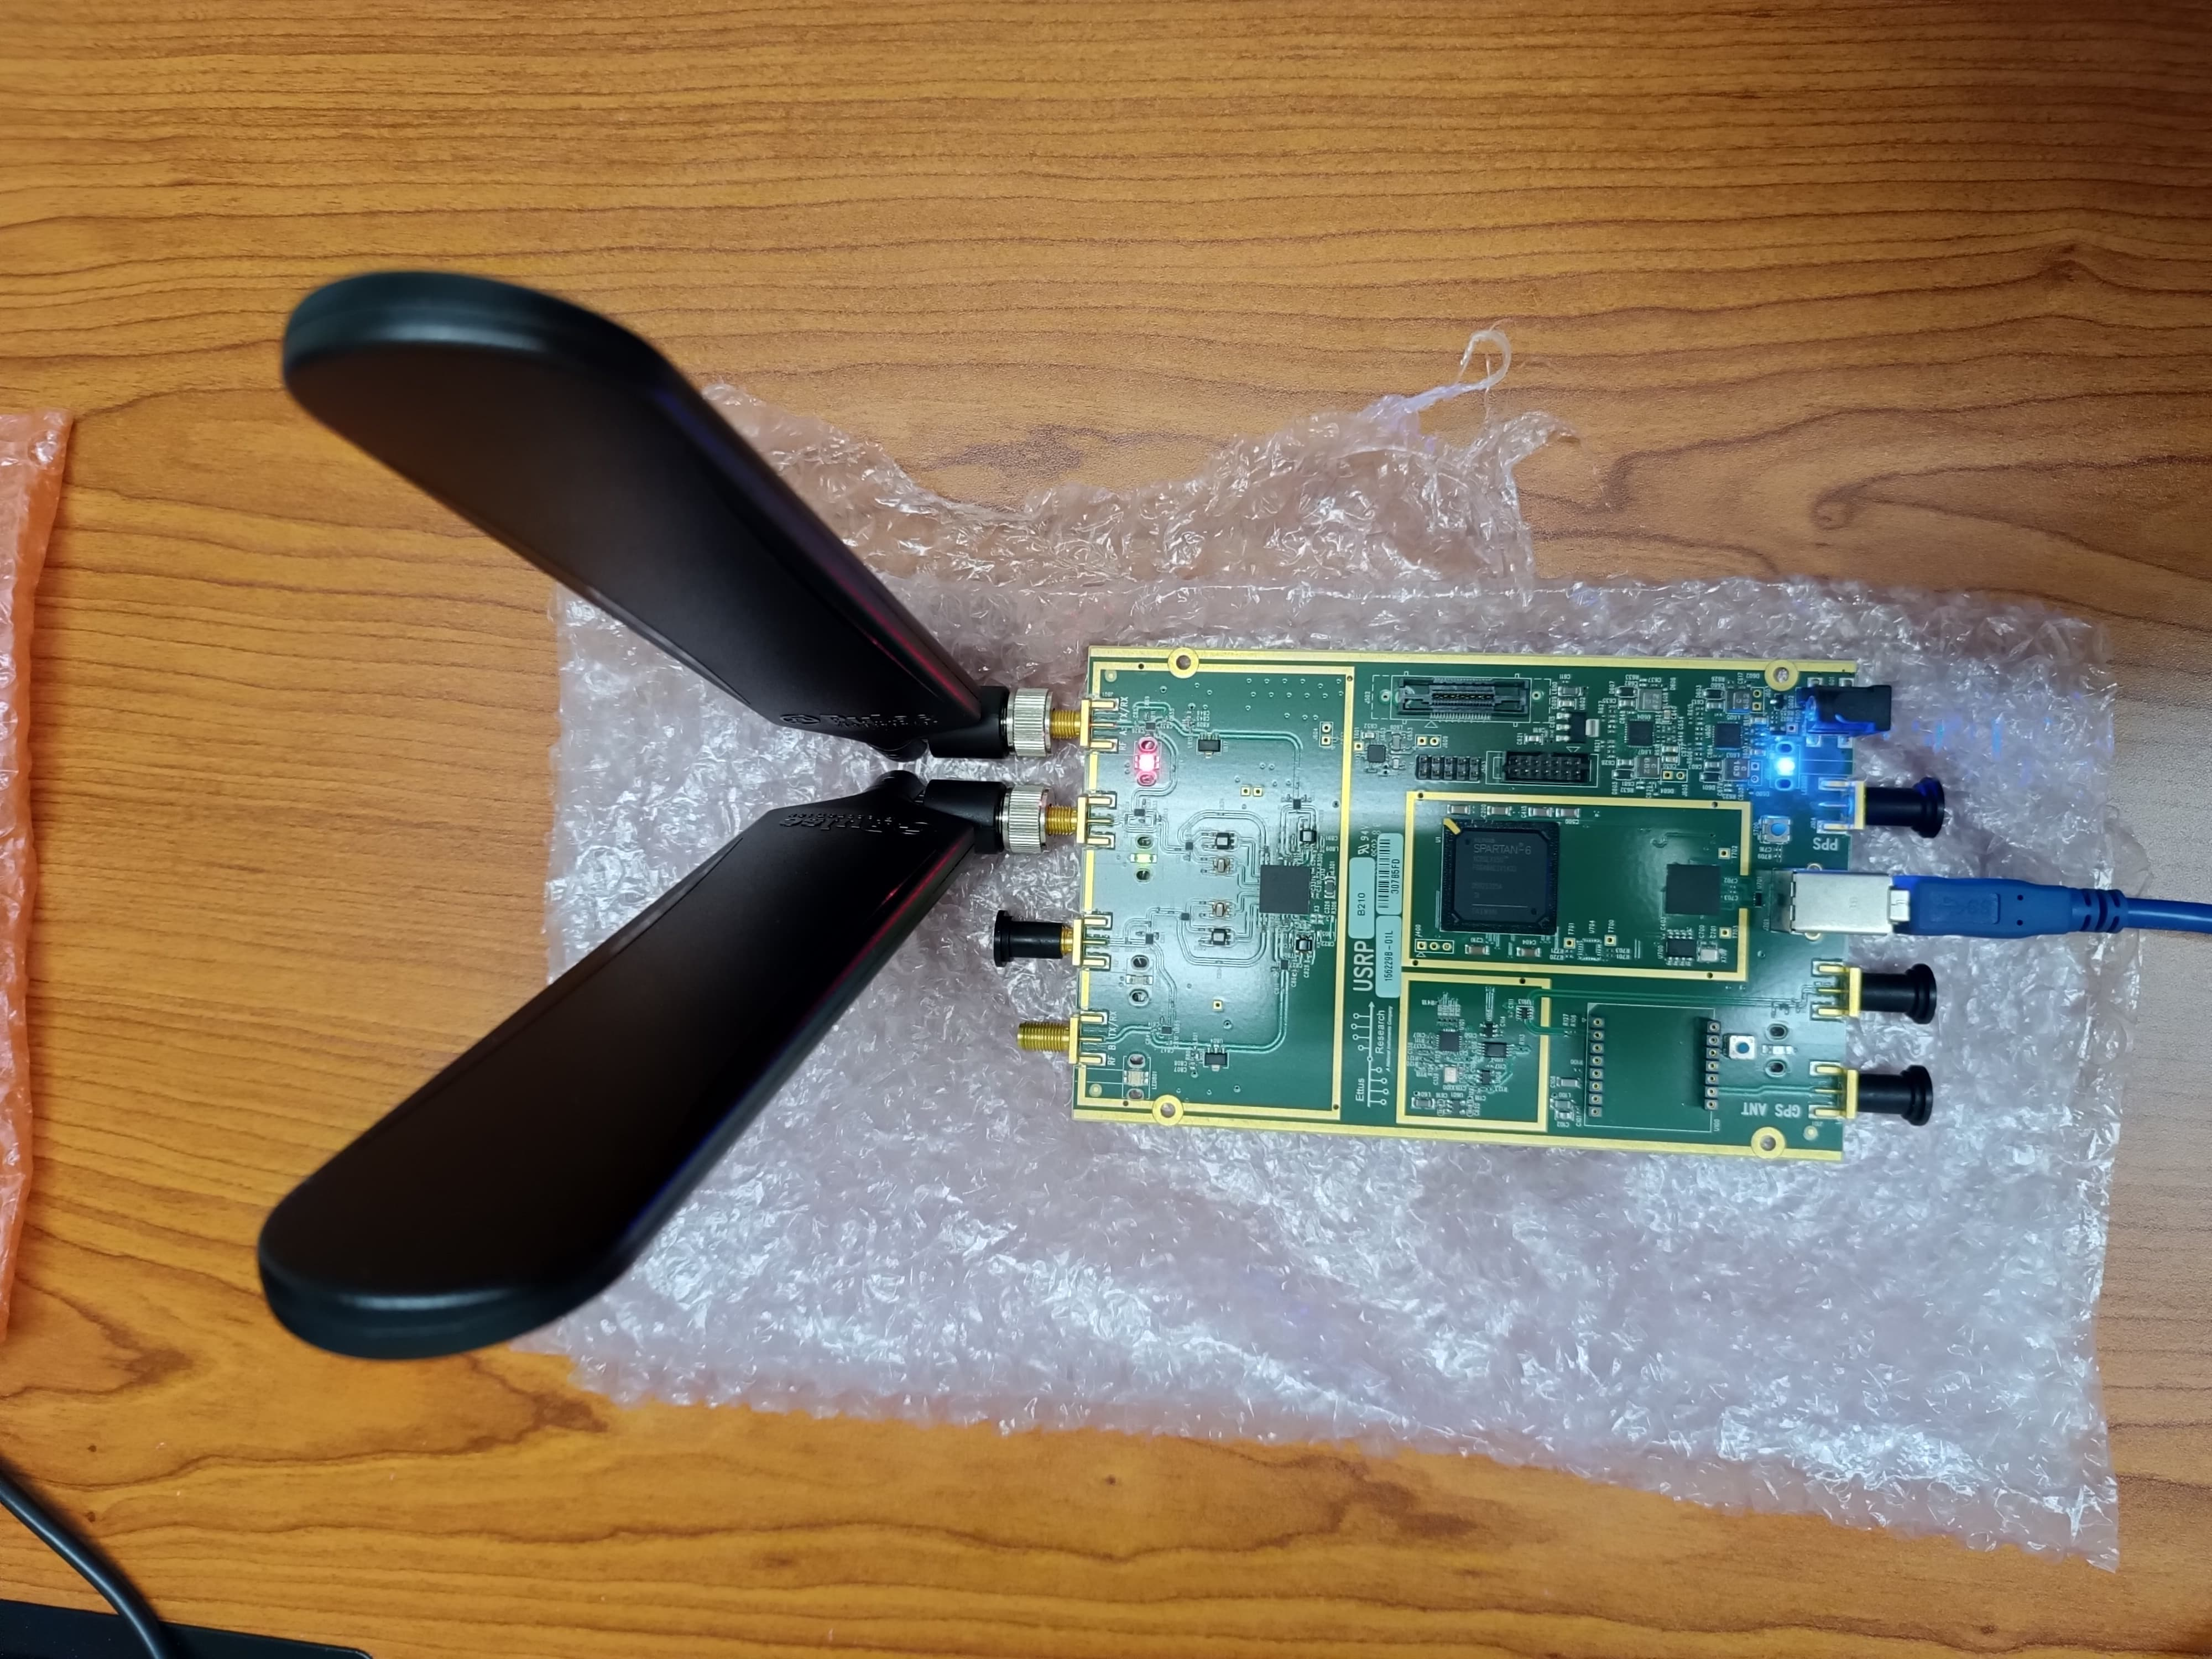
\includegraphics[width=0.5\linewidth]{figures/usrp_working}
    \caption[USRP B210 SDR operating]{USRP B210 SDR operating.}
    \label{fig:usrp_working}
\end{figure}

To ensure the correct registering in the Core Network, it is necessary to check the packet exchange between gNB and Core, using Wireshark.
Figure~\ref{fig:gnb_reg} presents the successful registration of the gNB with the AMF\@.

\begin{figure}[H]
    \centering
    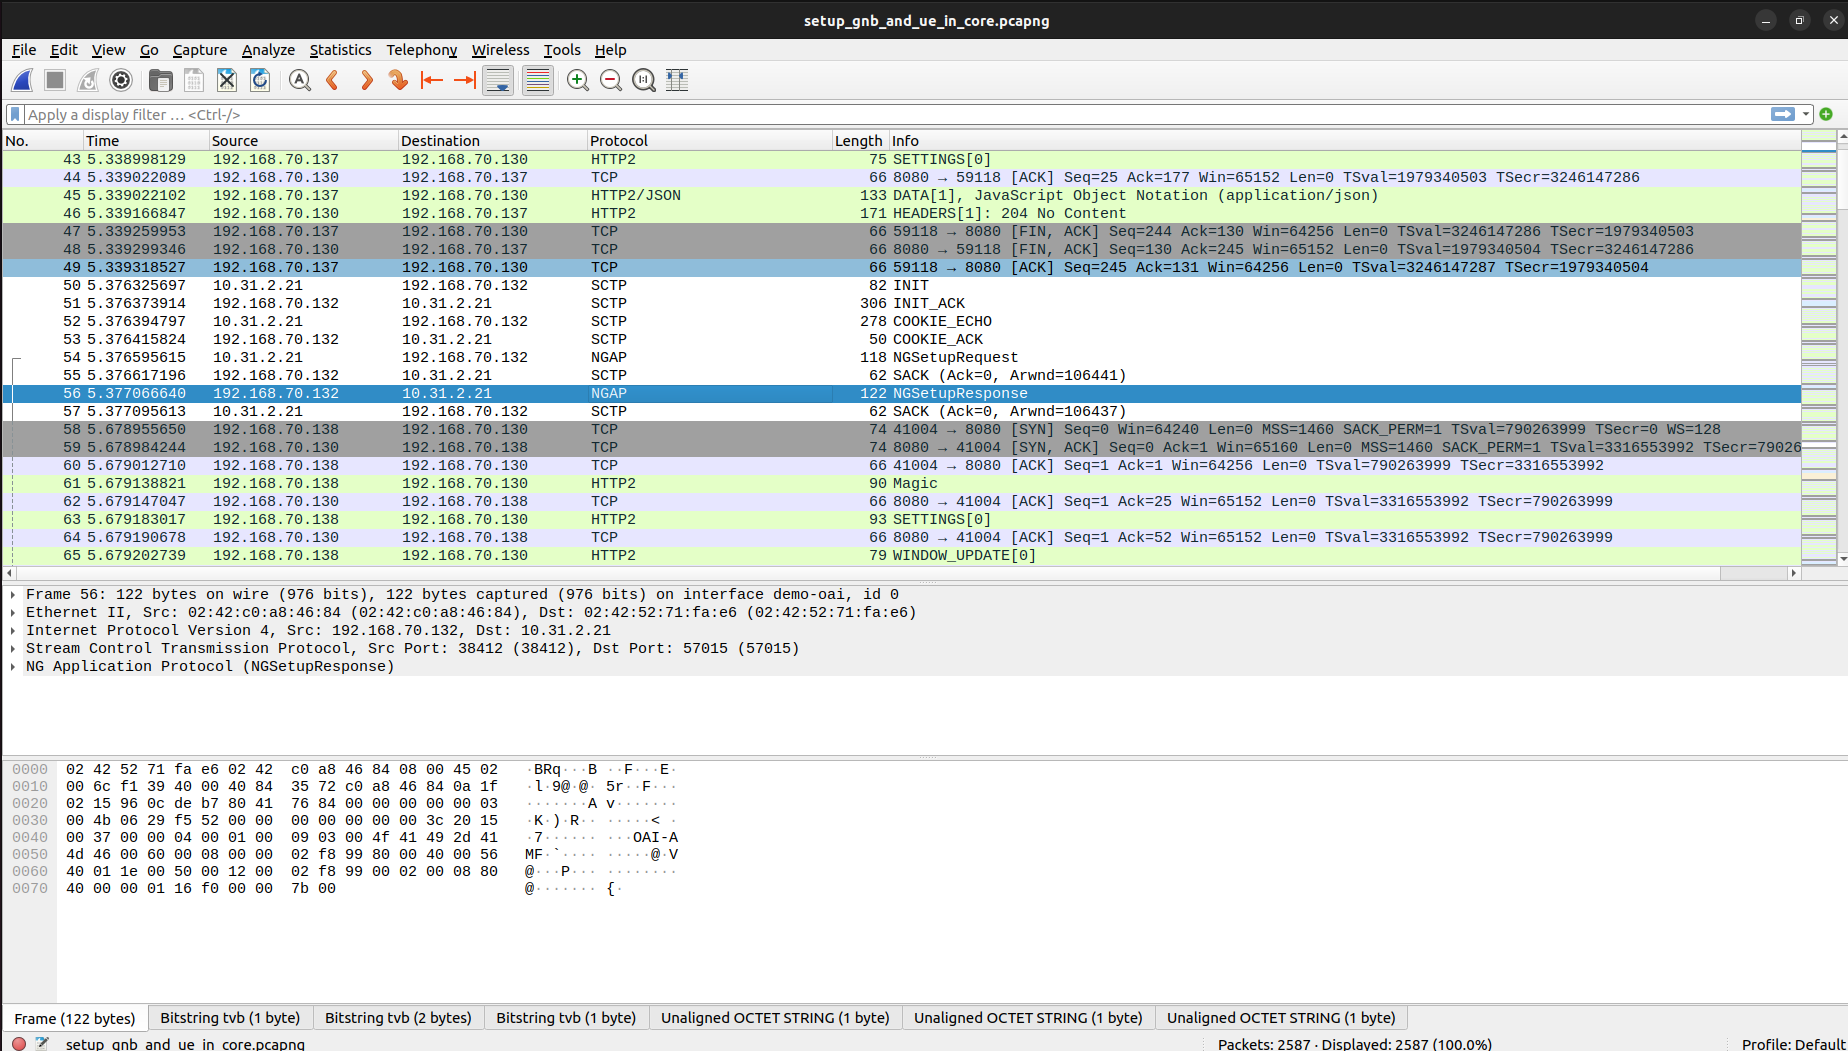
\includegraphics[width=0.5\linewidth]{figures/register_gnb}
    \caption[gNB registering via N2 interface]{gNB registering via N2 interface.}
    \label{fig:gnb_reg}
\end{figure}

The final verification is to check the connection between FlexRIC and gNB through E2 interface.
This is possible to observer in the terminal running FlexRIC, where logs show the registration.
Figure~\ref{fig:gnb_e2} shows this registration.

\begin{figure}[H]
    \centering
    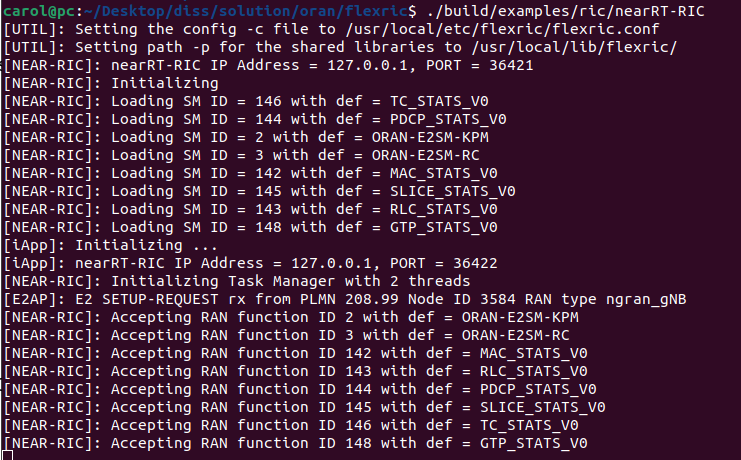
\includegraphics[width=0.5\linewidth]{figures/gnb_e2_flexric}
    \caption[gNB's E2 node registering with FlexRIC]{gNB's E2 node registering with FlexRIC.}
    \label{fig:gnb_e2}
\end{figure}

\subsection{UE}\label{subsec:ue}

In order to test the correct initialization of the UE we needed to ensure connection with the Core Network.
After executing the command present in~\ref{subsec:oai-5g-ue}, we observed in Wireshark the correct registration of the UE in Figure~\ref{fig:registration_ue}.

\begin{figure}[H]
    \centering
    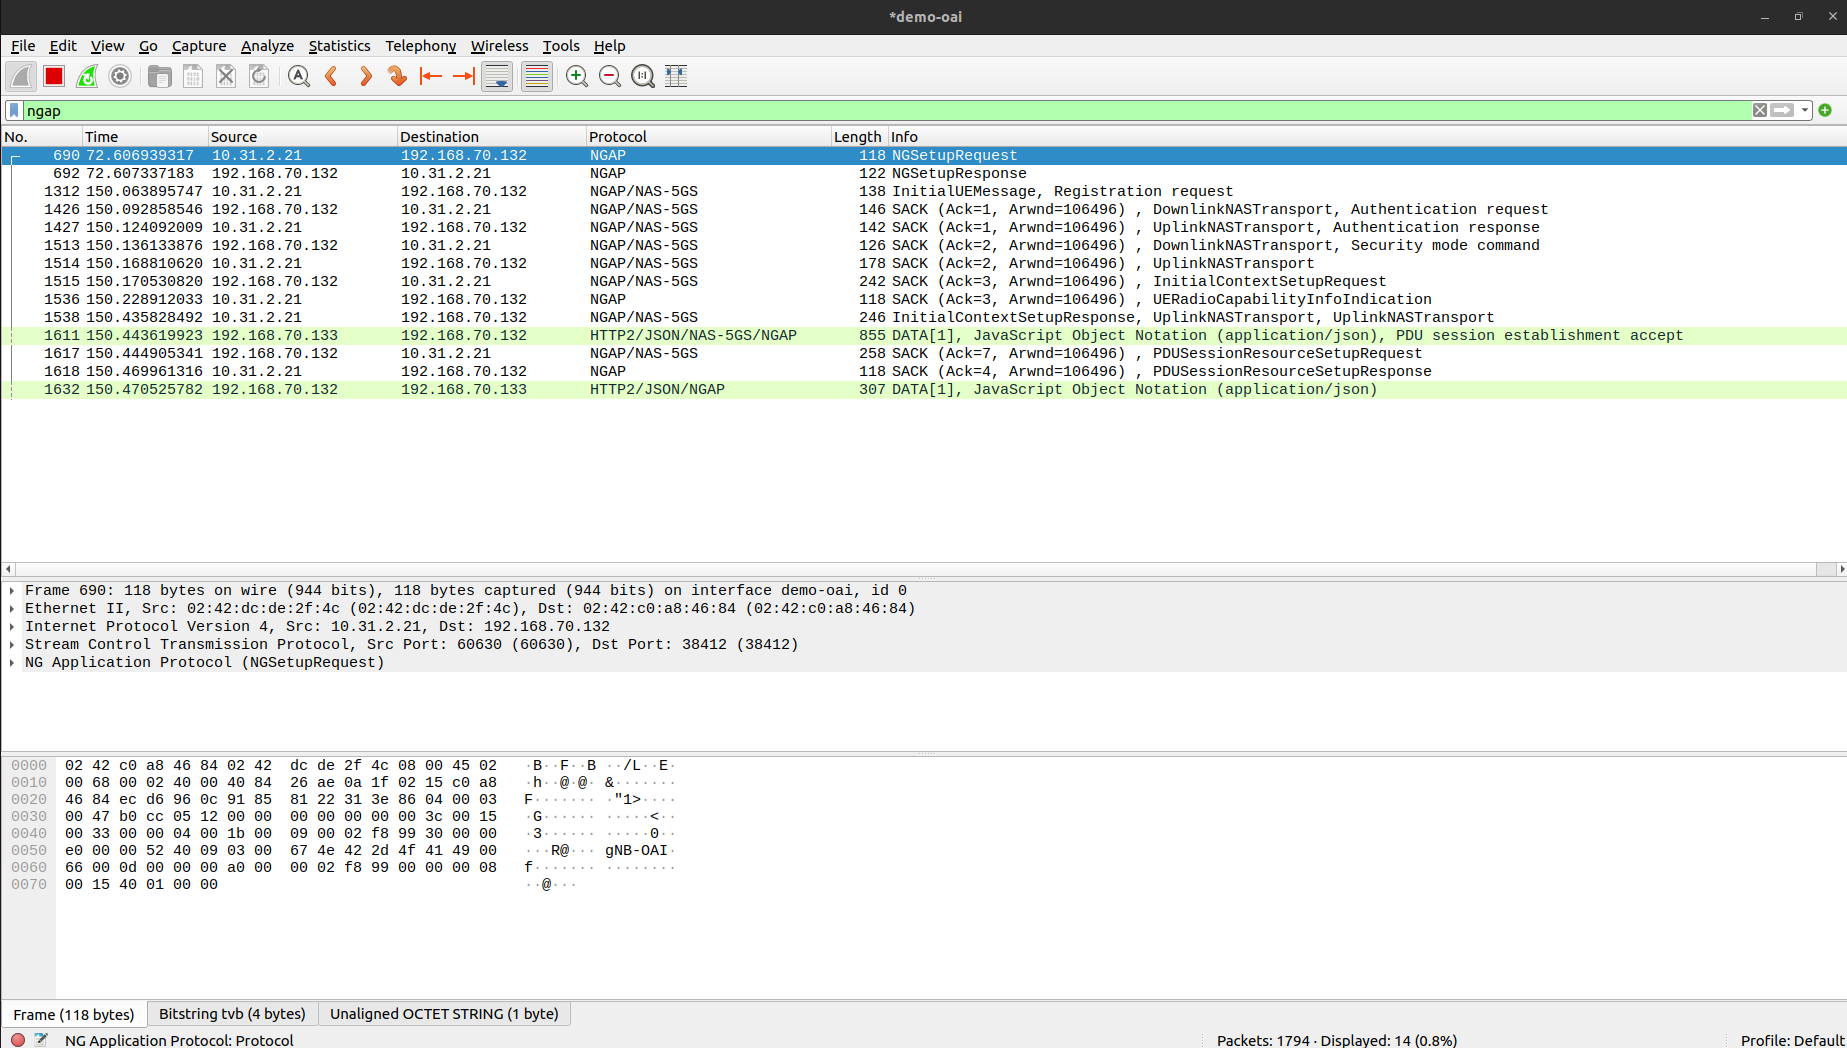
\includegraphics[width=0.5\linewidth]{figures/ue_registration}
    \caption{Registration of the UE.}
    \label{fig:registration_ue}
\end{figure}

When this synchronization occurs, we can verify the creation of \textit{oaitun\_ue1}, the tunnel interface between UE and Core Network.
With that, we can test its connectivity, by pinging to every Core Network component, as well as the Internet.
Figures~\ref{fig:ping_ue_core} and~\ref{fig:ping_ue_internet} shows the outcome of these tests, to Core and to the Internet respectively.

\begin{figure}[H]
    \centering
    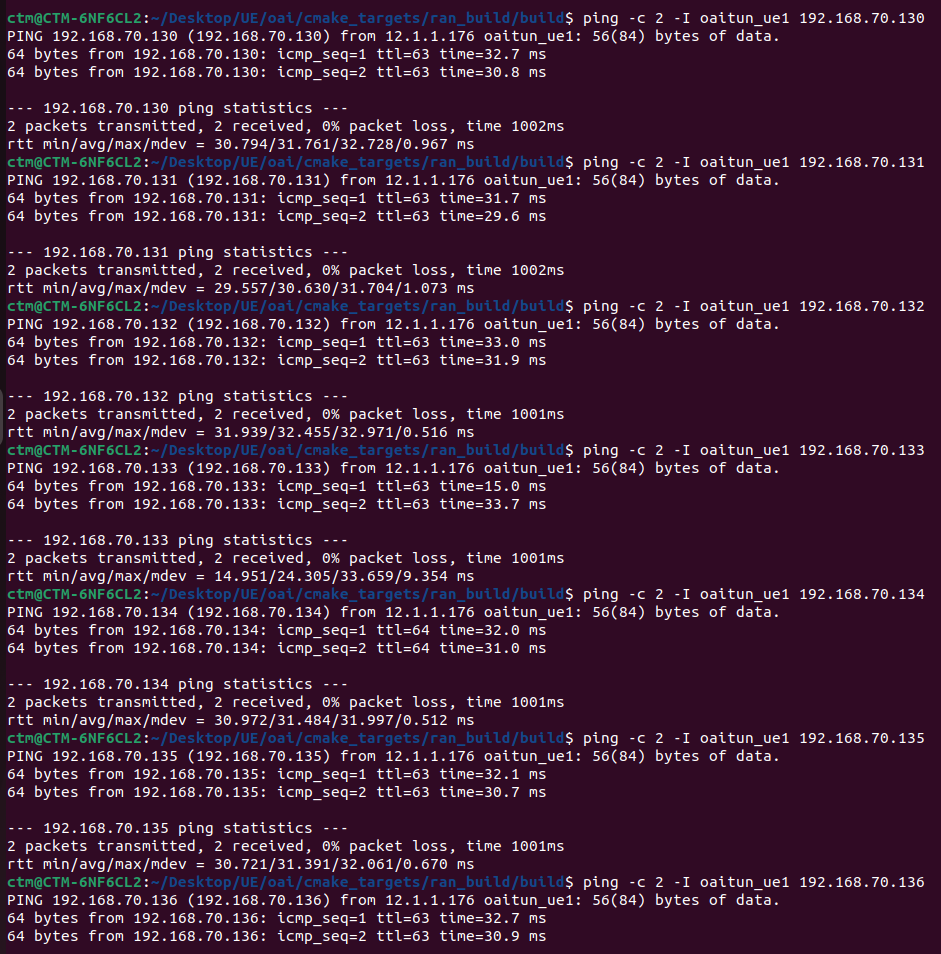
\includegraphics[width=0.5\linewidth]{figures/ue_core_ping}
    \caption{Pinging from UE to the Core Components.}
    \label{fig:ping_ue_core}
\end{figure}

\begin{figure}[H]
    \centering
    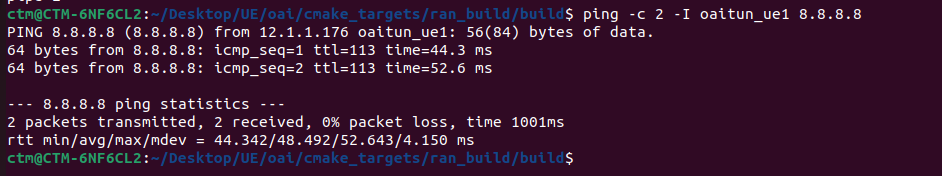
\includegraphics[width=0.5\linewidth]{figures/ue_to_ext}
    \caption{Pinging from UE to Google's public DNS server.}
    \label{fig:ping_ue_internet}
\end{figure}


\subsection{Vision Module}\label{subsec:cv_module}
To ensure the correctness and reliability of the VM, a series of validation tests were conducted.
These tests were designed to evaluate both the processing capabilities of the module and the accuracy of the message exchange between the VM and the xApp.

The time for processing a frame varies according to some factors, such as the complexity (i.e.\ number of objects present) and the temporal variation of the scene.
This implicates in design choices such as the periodicity of extraction of metrics by the xApp.
The processing time of each frame was measured to assess the performance of the VM\@.
The average processing time, testing with real-time capturing is 5 FPS\@.
While this is 17\% of the frame capture rate, this value is sufficient to evaluate if our solution allows the adaptation of the gNB\@.

A reference video was used to evaluate the detection and tracking results of the VM\@.
This video, containing people walking, was processed to check for detection accuracy and tracking consistency.
It was confirmed that the module could accurately detect and track objects, validating its effectiveness in a real-world scenario.
Figure~\ref{fig:reference_video} shows a capture of such video, as well as the encoded and decoded messages generated.

% image of a frame of the video and the corresponding messages
\textcolor{red}{UPDATE IMAGE}
\begin{figure}[H]
    \centering
    
\includegraphics[width=0.5\linewidth]{figures/uporto-feup}
    \caption{Reference video and corresponding messages generated.}
    \label{fig:reference_video}
\end{figure}

Print statements were used on the server side to verify the correct formatting, coding, and decoding of the messages.
This step was crucial to ensure that the messages sent from the module to the xApp were correctly structured and could be properly interpreted upon receipt.

On the client side,the xApp, print statements were employed to confirm the correct reception of the messages.
This validation step ensured that the messages transmitted through the socket connection were properly received and could be correctly processed.

To further validate the communication, Wireshark was used to capture SCTP packets containing the messages exchanged between the server and client, shown in Figure~\ref{fig:capture_messages}.
This capture provided a view of the message flow, confirming that the messages were being transmitted as expected without any loss or corruption.

\begin{figure}[H]
    \centering
    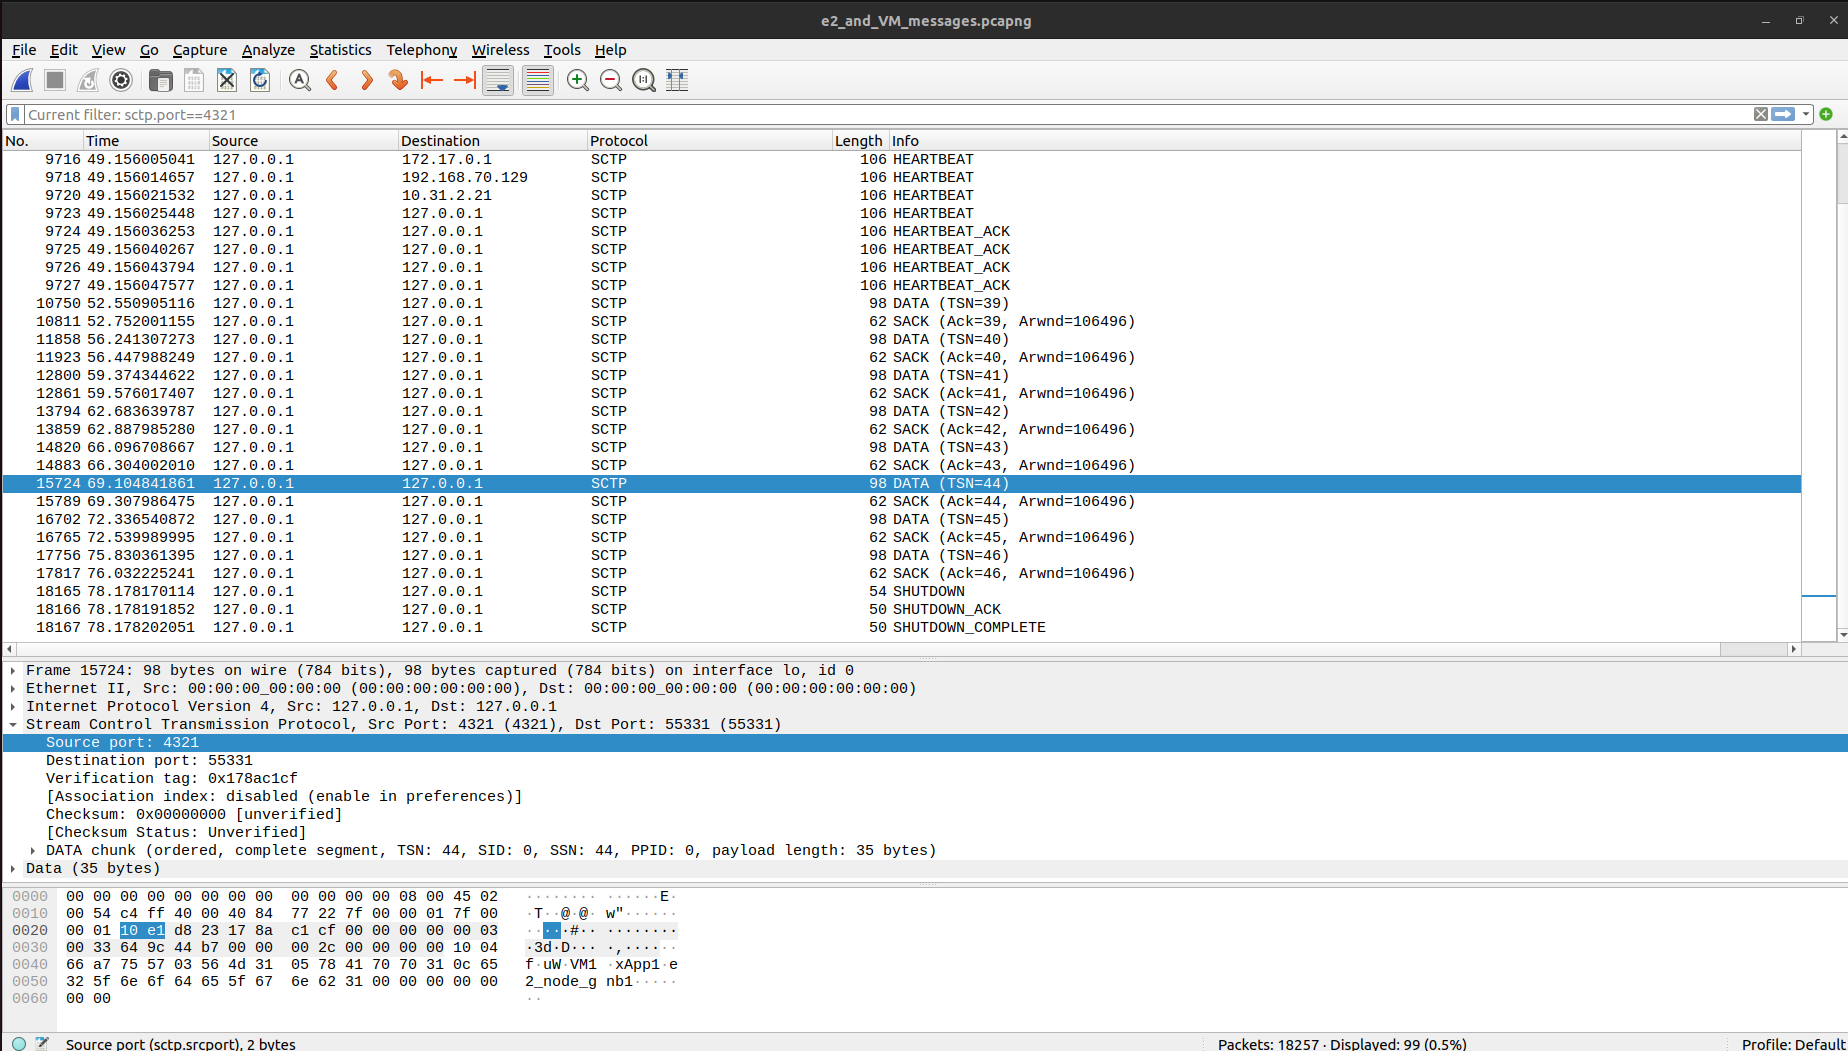
\includegraphics[width=0.5\linewidth]{figures/vm_xapp}
    \caption[SCTP packet exchange between VM and xApp]{SCTP packet exchange between VM and xApp.}
    \label{fig:capture_messages}
\end{figure}

The VM's performance proved adequate for the intended application, i.e.\ an indoor environment where movements are frequent yet the velocity is low, such as people walking or objects being moved.
The module demonstrated good performance in these scenarios, and its near real-time processing capability can trigger prompt reactions to environmental changes.

\subsection{xApp}\label{subsec:mm_xapp}
After all components of our system were deployed, and properly functioning, we accessed the correct functioning of the xApp.
The first verification is to access if the xApp could communicate with the FlexRIC software.
This allows the E2 subscription to the E2 node on the gNB, in order to retrieve data from it.
Figure~\ref{fig:xapp_subscription} shows this process.

\begin{figure}[H]
    \centering
    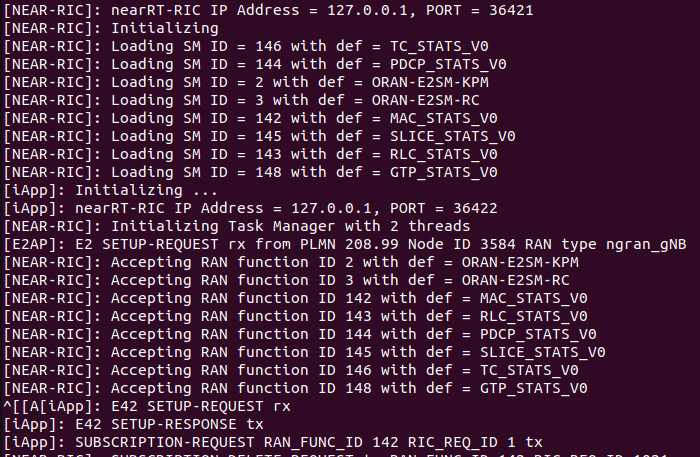
\includegraphics[width=0.5\linewidth]{figures/xapp_subscription}
    \caption{FlexRIC receiving the subscription request from the xApp.}
    \label{fig:xapp_subscription}
\end{figure}

E2 indication messages are received by the xApp once this subscription process is concluded.
The periodicity of such messages can be defined in the xApp.
We chose to receive each 10ms, Medium Access Control (MAC) layer metrics, in order to obtain SNR measurements.
Those values are essential for the state machine described in Section~\ref{subsec:xapp}.
The E2 subscription procedure can be seen in Figure~\ref{fig:captura_e2ap}.

\begin{figure}[H]
    \centering
    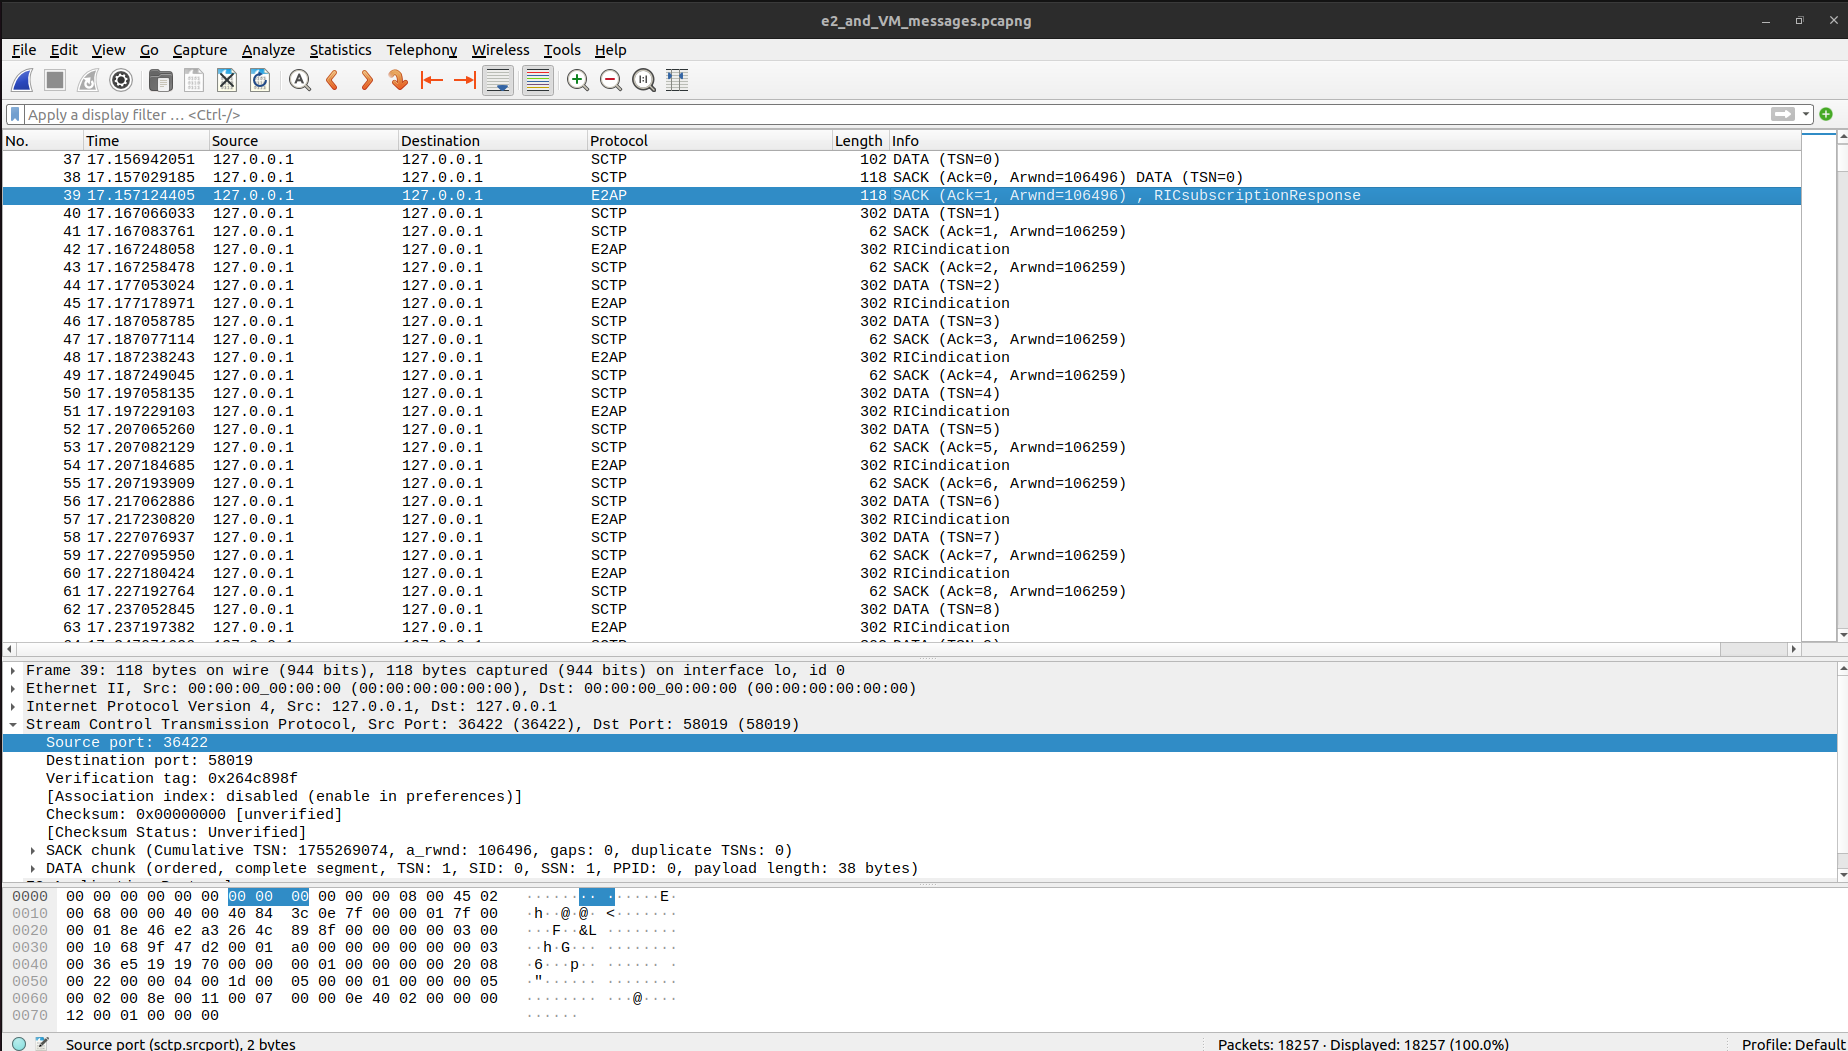
\includegraphics[width=0.5\linewidth]{figures/ric_subs}
    \caption{E2 Subscription Response and E2 Indication messages.}
    \label{fig:captura_e2ap}
\end{figure}

\section{Use case}\label{sec:use_case}
In order to validate the implemented solution, a use case testing scenario was established.
In an indoor environment, the system followed the architecture presented in Figure~\ref{fig:my_arch}.

The goal of test was to access the functionality of the whole system, considering maintaining channel quality, or increasing it whenever possible.
The xApp suggests the repositioning of the gNB, based on data collected from the Vision Module and the RF metrics collected from the RAN via the Near-RT RIC\@.

The use case shows the system's capabilities in four test scenarios, described in the following subsections.

For all scenarios we are assuming constant velocity for all moving entities.

\subsection{Scenario 0 : Fixed gNB and UE}\label{subsec:scenario-0-:-fixed-gnb-and-ue}

In this scenario, the objective is to assess the impact of blockages on the LoS between the gNB and the UE\@.
By maintaining a fixed position for both the gNB and the UE, we can introduce obstacles to observe their effects on signal quality.
This scenario also aims to validate the accuracy of the messages sent by the vision module regarding the presence of blockages.
Figure~\ref{fig:test_fixed} presents a top-view from the testing scenario.
The obstacle moves from left to right, over time at a constant velocity.

The results from this scenario serve as a baseline for comparison with other scenarios, where the positions of the gNB and UE may vary.
This analysis is important for evaluating the gains of having CV solutions integrated into mobile networks.

\begin{figure}[H]
    \centering
    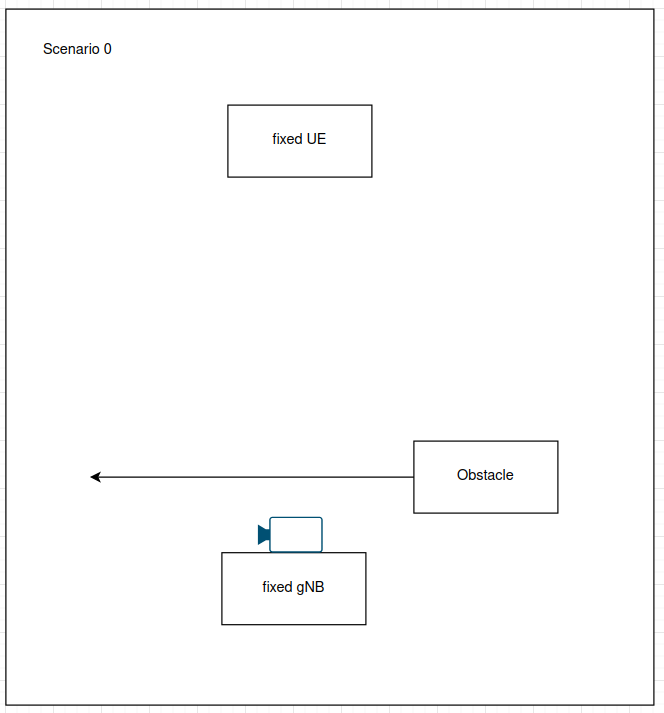
\includegraphics[width=0.5\linewidth]{figures/scenario0}
    \caption{Overview of the movement for scenario 0.}
    \label{fig:test_fixed}
\end{figure}

\begin{figure}[H]
    \centering
    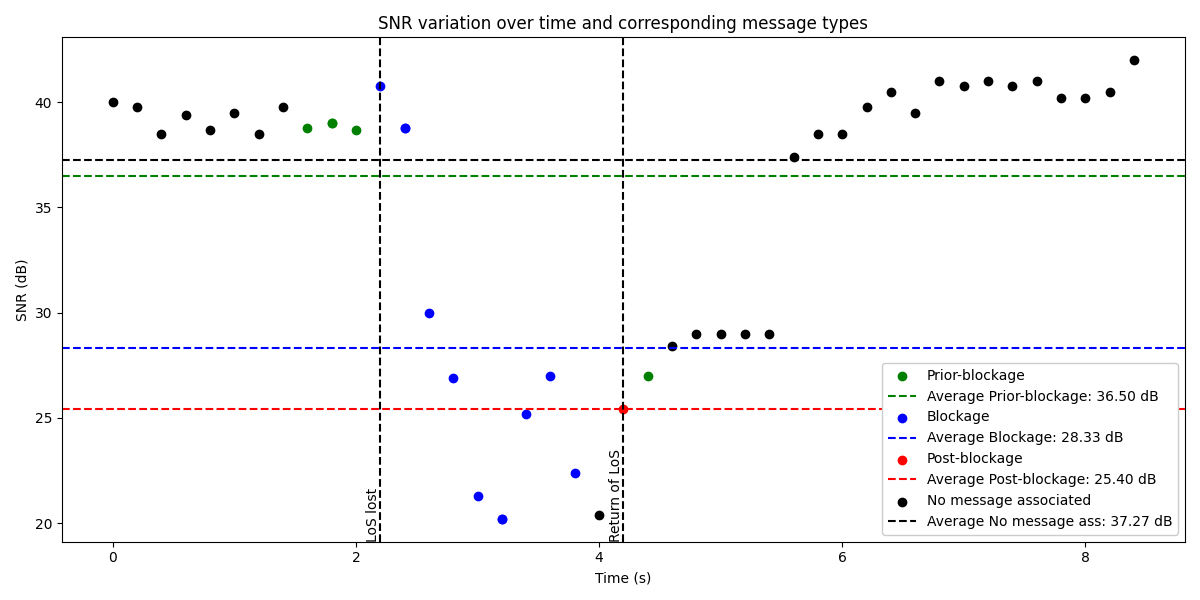
\includegraphics[width=\linewidth]{figures/results_0}
    \caption{SNR variation over time and the respective VM messages for scenario 0.}
    \label{fig:results_0}
\end{figure}


This test was successful, showcasing the CV module messages received, as well as SNR metrics corresponding to those expected.

Figure~\ref{fig:results_0} presents the graph with the results collected from this experiment.
It is possible to see the SNR variation over time in the y-axis , associated with each message.
The average SNR values are collected by the xApp in intervals of 200 milliseconds (20 sample collected over a period of 10ms).
Possible values for this collection of data are 1ms,2ms, 5ms or 10ms.
This value is set according to the estimated processing framerate of the video.
Since prior test has shown that capturing in 30 fps results in the processing of video of about 5fps, we chose this value so that each message reception will have an SNR associated.
Each message is represented by a colour, as shown in the legend.
Notice that we can also have situations were we have SNR data collection but no associated message, for instance when no obstacles are detected or when the obstacles seen are not expected to block the LoS\@.

The graph is divided into three distinct stages, separated by the transition lines.
In the first stage, where the obstacle is moving towards the UE, Prior Blockage messages are sent.
The SNR is high  since there is no obstruction of LoS between gNB and UE, indicating a strong and clean signal.

The first transition is labeled \('\)LoS lost\('\).
This marks the beginning of the blockage period.

In the second stage,the obstacle stops in front of UE, and it is possible to see the reception of the first Blockage Message, indicating the beginning of such obstruction.
As expected, the average SNR lowers.

The second transition is labeled \('\)Return of LoS\('\), indicating the end of the blockage and the return to normal signal conditions.
In the third stage, the obstacle moves away from the UE, no longer blocking the LoS\@.
As expected, the average SNR approximate those seen in the first stage.
The SNR values increase, similar to the prior blockage stage, indicating the restoration of a clear and strong signal, suggesting the passage of the blockage.

In this scenario, we also have used iperf tool to test the throughput in two instants.
The first one was when no blockage was occurring.
The second on was when a blockage was ongoing.
This test was using TCP packets and assessed the throughput of the uplink.
As expected, the throughput is lower when there is a blockage.
Table~\ref{tab:iperf} presents the measured values.


\begin{table}[h]
    \centering % Center the table
    \begin{tabular}{|c|c|c|c|}
        \hline
        \textbf{Instant} & \textbf{Throughput} \\ \hline
        No blockage & 936 kB \\ \hline
        Blockage   &  643 kB\\ \hline
    \end{tabular}
    \caption{Iperf results for LoS and NLoS} % Add a caption for the table
    \label{tab:iperf} % Add a label for referencing the table
\end{table}


\subsection{Scenario 1: Fixed gNB, moving UE}\label{subsec:scenario-0.1:-fixed-gnb-moving-ue}

In this scenario, the objective is to assess the limitations of our VM and characterize the messages' occurrence\@.
We seek to access how the vision-aided gNB behaves when there is a moving UE\@.
The UE is being carried by a person and the VM model can detect both the person and the UE\@.
Figure~\ref{fig:test_movUE} presents a top-view from the testing scenario.
The UE moves from left to right, over time at a constant velocity.

\begin{figure}[H]
    \centering
    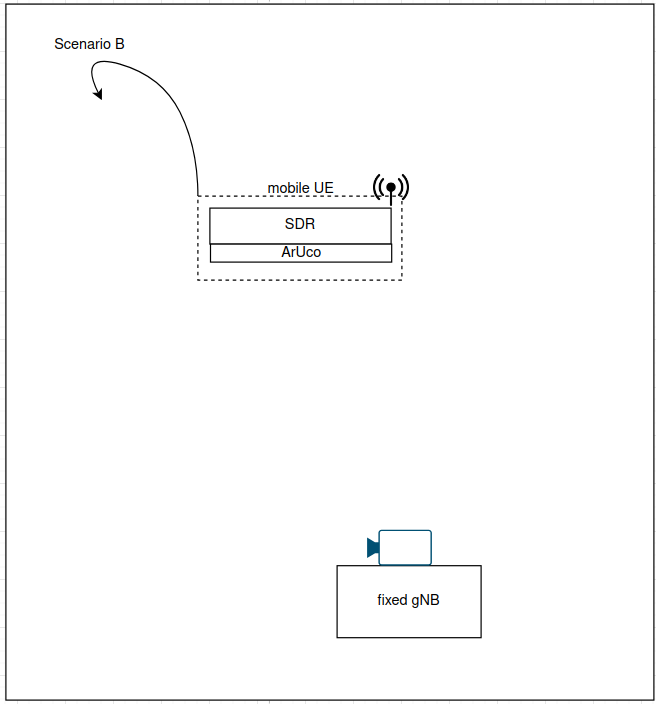
\includegraphics[width=0.5\linewidth]{figures/scenario1}
    \caption{Overview of the movement for scenario 1.}
    \label{fig:test_movUE}
\end{figure}

This test occurred as expected.
We noticed that the CV module generated wrong messages specially when it came to Pior Blockage messages, as anticipated.
This is due to the fact that the module has no notion of depth.
It interprets the person as an obstacle and calculates that the bounding box movement of the person will intersect with the UE's.

Despite this limitation, it is possible to notice that the VM does not emit Blockage messages, since the UE has LoS with the gNB\@.
In the same fashion, it does not emit Post Blockage messages.

Figure~\ref{fig:results_1} presents the graph with the results collected from this experiment.
It is possible to see the SNR variation over time in the y-axis , associated with each message.
Notice that there is a variation in the SNR since the distance between gNB and UE increased.
As them return to being closer, the SNR is restored.

Some Prior Blockage messages are associated with those SNRs, while no obstacle is expected to block the LoS\@.
The VM module is sending those messages because it views the person carrying the UE as an obstacle, and it is moving in the same direction as the UE\@.


\begin{figure}[H]
    \centering
    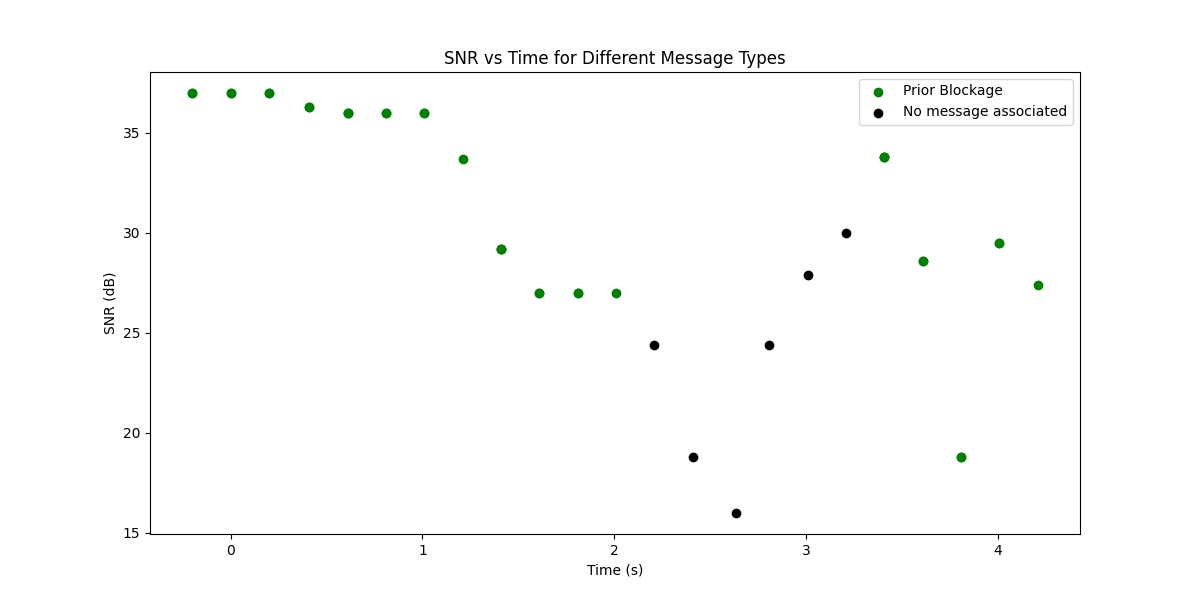
\includegraphics[width=\linewidth]{figures/results_1}
    \caption{SNR variation over time and the respective VM messages for scenario 1.}
    \label{fig:results_1}
\end{figure}

\subsection{Scenario 2: Fixed gNB, moving UE, Obstacle present}\label{subsec:scenario-0.1:-fixed-gnb-moving-ue-obstacle-present}

In this scenario, the objective is similar to the previous.
We seek to access how the vision-aided gNB behaves when there is a moving UE and multiple objects in the scene (a person carrying the UE and an obstacle represented by a person moving)\@.
The UE is being carried by a person and the VM model can detect both people and the UE\@.
Figure~\ref{fig:test_movUE} presents a top-view from the testing scenario.
The UE moves from left to right, over time at a constant velocity and the obstacle moves from right to left in the same fashion.

\begin{figure}[H]
    \centering
    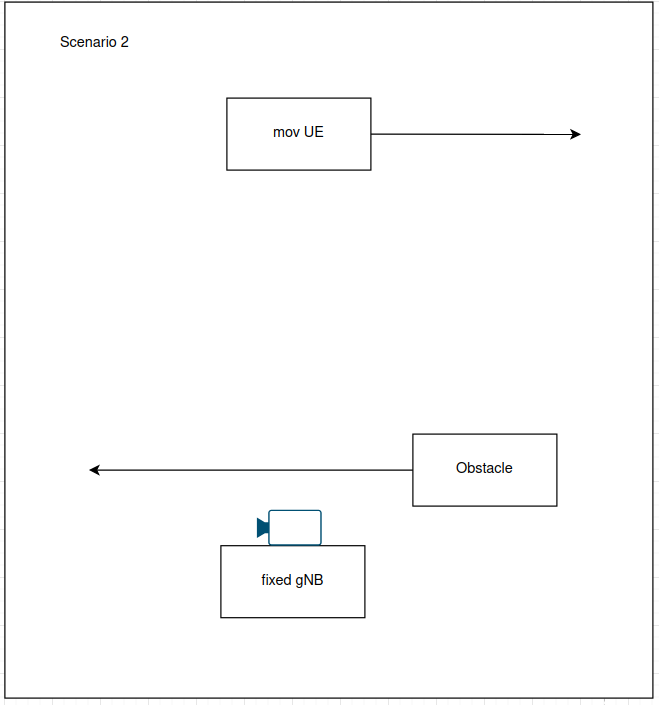
\includegraphics[width=0.5\linewidth]{figures/scenario2}
    \caption{Overview of the movement for scenario 2.}
    \label{fig:test_movUE_obst}
\end{figure}

This test occurred as expected.
As the previous scenario, the VM generated wrong messages specially when it came to Pior Blockage messages, as anticipated.
The difference from the previous scenario is that the VM still generates correct messages when it comes to the obstacle in the foreground of the frame.


Figure~\ref{fig:results_2} presents the graph with the results collected from this experiment.
It is possible to see the SNR variation over time in the y-axis , associated with each message.


\begin{figure}[H]
    \centering
    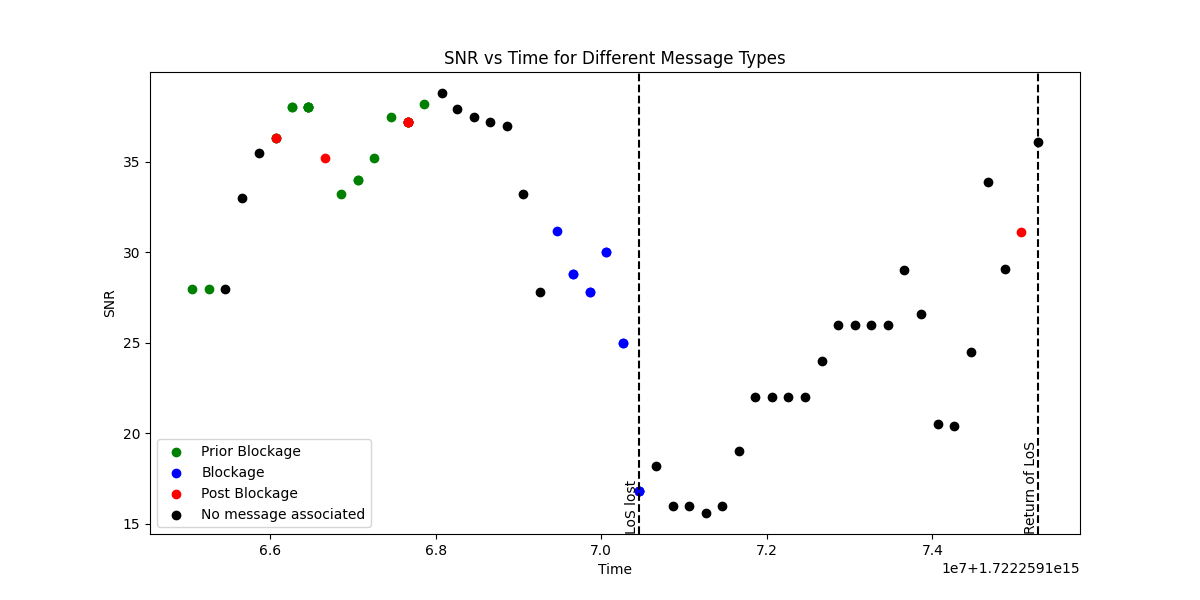
\includegraphics[width=\linewidth]{figures/results_2}
    \caption{SNR variation over time and the respective VM messages for scenario 2.}
    \label{fig:results_2}
\end{figure}

\subsection{Scenario 3: Moving gNB}\label{subsec:scenario-3:-moving-gnb}

In this scenario, the objective is to move the gNB in order to mantain LoS\@.
We seek to access the vision-aided gNB predictions and evaluate the benefits of moving a gNB\@.
The gNB is being moved in a table and the VM model can detect the obstacle and the UE\@.
Figure~\ref{fig:test_movgnb} presents a top-view from the testing scenario.
The UE  is fixed, the obstacle moves from right to left at constant pace and the gNB moves in the opposite direction.

\begin{figure}[H]
    \centering
    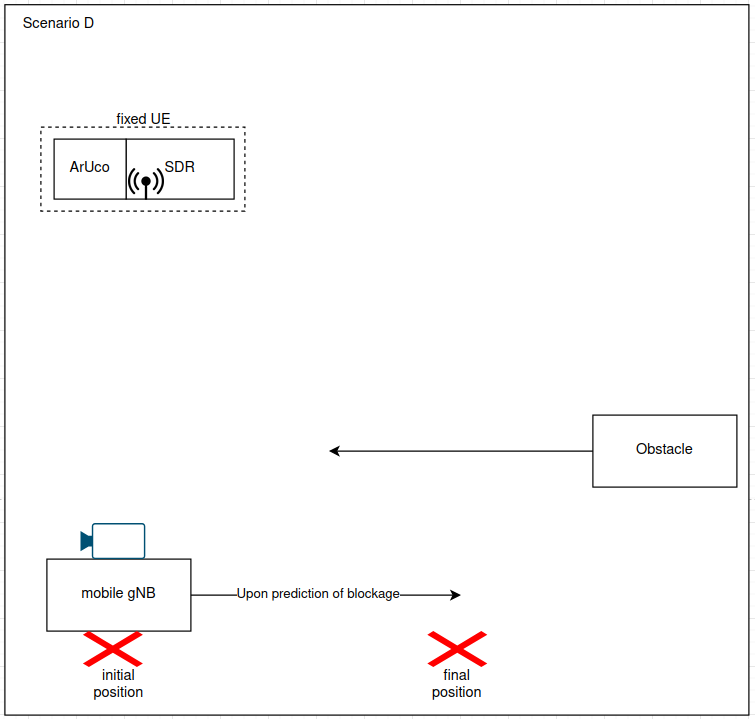
\includegraphics[width=0.5\linewidth]{figures/scenario3}
    \caption{Overview of the movement for scenario 3.}
    \label{fig:test_movgnb}
\end{figure}

Figure~\ref{fig:results_3} presents the graph with the results collected from this experiment.
It is possible to see the SNR variation over time in the y-axis , associated with each message.

Despite the limitations on the movement of the gNB in order to maintain the LoS, the test occurred as expected.
Such limitations are posed by the room where the tests were conducted, and for the SDRs limited range (about 2m), difficult the testing scenario.


\begin{figure}[H]
    \centering
    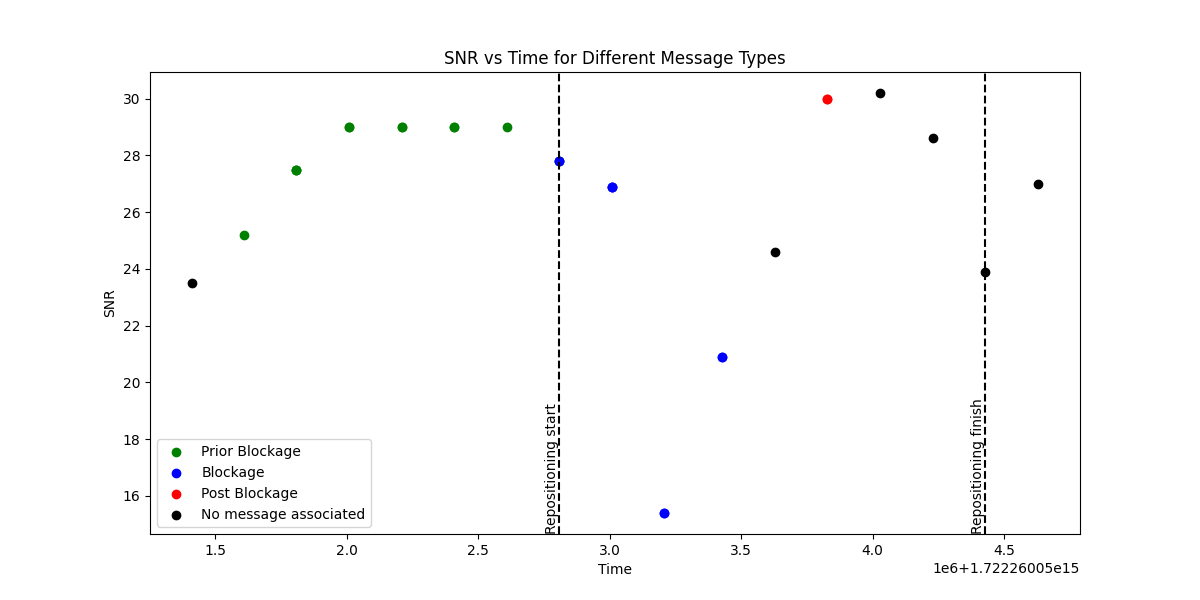
\includegraphics[width=\linewidth]{figures/results_3}
    \caption{SNR variation over time and the respective VM messages for scenario 3.}
    \label{fig:results_3}
\end{figure}

%\subsection{Scenario 2: UE Moving Away from the gNB}\label{subsec:scenario-2:-ue-moving-away-from-the-gnb}

%This scenario involves the UE moving progressively further from the gNB. In the absence of identified obstacles, a decrease in the Signal-to-Noise Ratio (SNR) is interpreted as the UE increasing its distance from the gNB. To address this, the robotic platform, leveraging the Mobility Management xApp, dynamically moves towards the UE to uphold optimal communication quality.
%This adaptive response ensures that the UE remains within the effective communication range of the gNB, thereby maintaining robust and reliable connectivity.


\section{Discussion}\label{sec:discuss}
The tests conducted successfully validated the proposed solution, demonstrating that the objectives of this dissertation were achieved.

Component tests confirmed the operational status of all individual entities, ensuring each part of the system functioned correctly.
Interoperability tests verified the integration of these entities, confirming that the system operates cohesively as a whole.
The evaluation demonstrated the viability of the proposed solution, indicating its potential for application in real-world scenarios.

The use of O-RAN facilitates the introduction of technologies within the RAN\@.
Specifically, the use of an xApp to incorporate CV messages, thereby enhancing RAN performance.
This integration showcases the flexibility and potential of O-RAN in enabling innovative solutions that improve network capabilities.
